\documentclass[10 pt]{article}
\usepackage[a4paper, total={7in, 9.5in}]{geometry}
\usepackage[spanish]{babel}
\usepackage{csquotes}
\usepackage{graphicx} 
\usepackage{caption}
\usepackage{hyperref}
\usepackage{graphicx}
\usepackage{float}
\usepackage{url}
\usepackage{color}
\usepackage{siunitx}
\usepackage{hhline}
\usepackage{multirow}
\usepackage[round]{natbib}
\bibliographystyle{plainnat}
\usepackage{todonotes}
\linespread{1.5}
\usepackage{imakeidx}
\makeindex[columns=3, title=Alphabetical Index, intoc]

\begin{document}




\listoftodos

\begin{titlepage}

    \begin{center}
    \vspace*{-0.5in}
    \begin{figure}[htb]
    \begin{center}
    
\includegraphics[scale=.3]{images/uba2.jpg}
    \end{center}
    \end{figure}
    
    \begin{large}
    Maestría en Explotación de Datos y Descubrimiento del Conocimiento\\
    \vspace*{0.15in}
    Universidad de Buenos Aires \\
    
    \vspace*{0.6in}
    \end{large}
    
    \begin{large}
    Trabajo integrador\\
    
    
    \end{large}
    \vspace*{0.2in}
    \vspace*{0.3in}
    
    
    \vspace*{0.3in}
    \rule{80mm}{0.1mm}\\
    \vspace*{0.1in}
    \begin{large}
    Victoria Colombo
    
    \vspace*{0.3in}
    
    \vspace*{0.1in}fecha
    \end{large}
    \end{center}
    
    \end{titlepage}

\newpage

\begin{abstract}


\end{abstract}
\newpage
\tableofcontents
\newpage

\section*{Introducción}\label{intro}


La violencia sexual comprende una multiplicidad de conductas o intentos de conductas, que van desde actos hasta comentarios sexuales, dirigidos contra la sexualidad de otra persona de manera coercitiva. El trabajo con datos sobre violencia sexual presenta complicaciones porque los datos suelen ser escasos o presentar gran cantidad de faltantes \citetext{\citealp[p.~150]{ferris2002world}}. Uno de los motivos es que las víctimas o su entorno a menudo se rehúsan a denunciar o participar en encuestas sobre este tipo de agresiones, o proveen información incompleta. Esto puede deberse a la vergüenza y el estigma social frecuentemente asociado no solo con la violencia sexual sino con la sexualidad en general, pero también a la falta de acceso a la justicia, al temor a las represalias por parte de los agresores, o el temor a que la denuncia no sea creída \citep*{murphy2022unfounded}. Otros posibles motivos para la escasez y/o mala calidad de los datos pueden ser la falta de vías adecuadas para recabar esta información, o la negligencia o desconocimiento de procedimientos adecuados por parte de oficiales de policía encargados de recibir denuncias. A pesar de las dificultades en la recolección de datos, diversos estudios a nivel mundial logran identificar patrones frecuentes en la violencia sexual. Para este trabajo, resultan relevantes dos de ellos: la mayoría de las víctimas son mujeres, mientras que los perpetradores suelen ser hombres \citetext{\citealp[p.~149]{ferris2002world}; \citealp[p.~15]{contreras2016violencia}}; y en la mayoría de los casos, los agresores son personas conocidas por las víctimas, como parejas, exparejas u otros conocidos \citetext{\citealp[p.~9]{garcia2005multi},\citealp[p.~22]{unicef2018analisis}, \citealp[p.~151]{ferris2002world}}.
 
La clasificación de las identidades de género de víctimas y perpetradores es compleja. Por un lado, muchos estudios clasifican a las personas únicamente como hombres o mujeres, omitiendo las identidades de género disidentes.\footnote{Entre los estudios e informes consultados para este trabajo, solamente el \textit{Relevamiento de fuentes secundarias de datos sobre violencia sexual} de la \citet{ufem_relevamiento} menciona identidades de género cuando especifica que la violencia sexual “afecta particularmente a las mujeres cis y personas LGBTI+” (p.7).}. Por otro lado, aunque se reportan pocos casos de violencia sexual contra hombres cisgénero, es probable que estén subrepresentados debido a los prejuicios y estigmas sociales sobre la masculinidad que dificultan las denuncias y el acceso a la justicia para estas víctimas \citep*[p.~149]{ferris2002world}. Analizar esas complejidades excede a este trabajo de especialización. En mi análisis las categorías de género de víctimas, victimarios y llamantes se limitan a las registradas en el \textit{dataset}: hombre, mujer, y transgénero, sin especificar si es un hombre o una mujer transgénero. Reconozco esto como una limitación no solo de mi trabajo sino también de los datos disponibles.  

La  recopilación, sistematización, y análisis de datos sobre violencia sexual por parte de los Estados es crucial para planificar y llevar adelante políticas efectivas de prevención, asistencia, y erradicación de la violencia sexual. En Argentina, si bien no hay un sistema estatal único y centralizado de este tipo de información, existen entidades judiciales y programas estatales que, además de ofrecer auxilio, asistencia y/o acceso a la justicia, recaban datos sobre violencia sexual, y mantienen un registro público de ellos. Unos de esos programas es Las Víctimas contra las Violencias. 

Desde el año 2016, en el marco del programa Las Víctimas contra las Violencias, dependiente del Ministerio de Justicia de la Nación, la línea 137 funciona las 24 horas del día para solicitar asistencia en casos de violencia sexual o familiar\footnote{Además, desde 2020 cuenta también con el canal de \textit{Whatsapp} (54911) 3133-1000.}. El programa cuenta con equipos de intervención de abogadas, psicólogas, y trabajadoras sociales. Al recibir una llamada solicitando asistencia se coordina el envío de equipos móviles para proveer a la víctima, en base a las necesidades del caso, de contención emocional, acompañamiento a un hospital y/o a radicar una denuncia, y/o a un lugar seguro donde pueda alojarse \citep*{linea_137}.\todo[inline]{rever cómo sigue el programa ahora}

Los registros de las llamadas a la línea 137 se encuentran digitalizados desde 2017 y están disponibles en el \href{http://datos.jus.gob.ar/}{Portal de Datos Abiertos de la Justicia Argentina}. Allí se encuentran publicados cuatro tipos de \textit{datasets} por año: llamados e intervenciones domiciliarias por situaciones de violencia familiar, y llamados e intervenciones domiciliarias por situaciones de violencia sexual.
Los registros no están exentos de los problemas frecuentes antes mencionados en los datos sobre violencia sexual, presentan información faltante de dos maneras: celdas vacías en el caso de las variables numéricas de edad, y respuestas NS/NC (no sabe-no contesta) en lugar de SI o NO en el resto de las variables categóricas. Teniendo en cuenta la clasificación de datos faltantes que se origina en \citet{rubin1976inference}, los datos faltantes en el \textit{dataset} de llamados son posiblemente del tipo \textit{missing at random} (MAR) y \textit{missing not at random/ non-ignorable missing data} (MNAR). Es decir, o bien los datos faltan por motivos que tienen que ver con otras variables (MAR), o bien el valor de los datos que faltan está relacionado con el motivo mismo por el que faltan (MNAR).\todo[inline]{quizás esto va en datos?}

En este trabajo analizo llamados para reportar violencia sexual a la línea 137 entre 2017 y 2021, e intento predecir valores faltantes de la variable “víctima convive con el agresor”. \todo[inline]{esto así declarado es una reverenda poronga}



\section*{Datos}\label{datos}

\subsection*{Obtención y limpieza}\label{limpieza}
Para este trabajo descargué del \href{http://datos.jus.gob.ar/}{Portal de Datos Abiertos} mencionado arriba 5 \textit{datasets} en formato \textit{csv} de llamados a la línea 137 para solicitar asistencia por violencia sexual. Los archivos pertenecen, a razón de uno de por año, al período entre enero de 2017 y julio de 2021. 

Una vez descargados, unifiqué los 5 archivos en un solo \textit{dataset}. Para eso fue necesario realizar una primera limpieza destinada a dejar consistentes los distintos archivos en términos de cantidad y nombre de columnas\footnote{La limpieza, normalización, y preprocesamiento del \textit{dataset} y la aplicación de los métodos exploratorios y predictivos fueron realizados en Python}:

\begin{itemize}
    \item Eliminé la variable \textit{caso\_id}, que solo existe a partir de 2020.
    \item Cambié el nombre de la variable \textit{llamado\_provincia\_indec\_id} en los \textit{datasets} de 2017, 2018, y 2019 a su equivalente en 2020 y 2021: \textit{llamado\_provincia\_id}.
\end{itemize}

El siguiente paso fue limpiar el \textit{dataset} unificado de inconsistencias y errores de carga varios: 
\begin{itemize}
    \item Unifiqué para todas las variables pertinentes los valores \textit{SI}, \textit{NO}, y \textit{NS/NC} dejándolos en mayúscula, ya que aparecían en distintos formatos: minúscula, mayúscula inicial, etc.
    \item Unifiqué en la variable \textit{victima\_vinculo\_agresor} el valor \textit{Ex pareja de la víctima} que aparecía también como \textit{Ex pareja}, \textit{Ex-pareja de la víctima} y \textit{Expareja de la víctima}, otro tanto hice con \textit{Pareja de la víctima} que presentaba variaciones similares.
    \item Unifiqué en \textit{hecho\_lugar} dos variaciones de una misma categoría: \textit{Otra institución}, y \textit{Otra Institución}, optando por la primera forma.
    \item Sustituí todos los valores \textit{Sin datos} por \textit{NS/NC} por considerarlos equivalentes.
    \item Quité espacios de comienzo y final de \textit{strings} para solucionar problemas del tipo \textit{Madre} =/= \textit{  Madre} 
    \item Convertí en la variable \textit{llamante\_vinculo} el valor \textit{Vecino} a \textit{Vecina/o}, ya que  no necesariamente se refiere unívocamente a personas de género masculino.
    \item Unifiqué en \textit{llamado\_provincia} “Ciudad Autónoma de Buenos Aires” y “CABA” optando por “CABA”. 
    \item Corregí en \textit{llamado\_provincia }las instancias de “Santa Fé” a “Santa Fe”.

\end{itemize}

\subsection*{Exploración}\label{exploración}

El \textit{dataset} final unificado consta de 19143 observaciones y 54 variables, en su mayoría categóricas, que aportan información sobre la víctima, el agresor, la persona que llama para reportar el hecho, el contexto del hecho y el tipo de violencia sufrida. En el cuadro \ref{tablavar} se puede ver un detalle de las variables y su tipo.

\begin{table}[H]
    \centering
    \caption{Resumen de las variables.}
    \label{tablavar}
    \begin{tabular}{|l|l|l|} 
    \hline
    \textbf{Descriptor} & \textbf{Tipo variable} & \textbf{Variable(s)}         
    \\ 
    \hline
    \multirow{2}{*}{Víctima} & Cuantitativa & victima\_edad 
    \\ 
    \cline{2-3}
     & Cualitativa & \begin{tabular}[c]{@{}l@{}}victima\_genero, victima\_nacionalidad, victima\_discapacidad, \\ victima\_vinculo\_agresor, victima\_convive\_agresor, victima\_a\_resguardo\end{tabular}          
     \\ 
    \hline
    \multirow{2}{*}{Llamante} & Cuantitativa         & {llamante\_edad}             
    \\ 
    \cline{2-3}
     & Cualitativa& llamante\_genero, llamante\_vinculo                  
     \\ 
    \hline
    \multirow{2}{*}{Llamado}& Ordinal & llamado\_fecha\_hora                                            
    \\ 
    \cline{2-3} & Cualitativa & \begin{tabular}[c]{@{}l@{}} caso\_id, llamado\_provincia llamado\_provincia\_id, \\ caso\_judicializado, hecho\_lugar\end{tabular}                                
    \\ 
    \hline
    Violencia sexual                 & Cualitativa  &  \begin{tabular}[c]{@{}l@{}} vs\_violacion\_via\_vaginal, vs\_violacion\_via\_anal, vs\_violacion\_via\_oral, \\ vs\_tentativa\_violacion, vs\_tocamiento\_sexual, vs\_intento\_tocamiento, \\ vs\_intento\_violacion\_tercera\_persona, vs\_grooming, vs\_exhibicionismo, \\ vs\_amenazas\_verbales\_contenido\_sexual, vs\_explotacion\_sexual,\\ vs\_explotacion\_sexual\_comercial, vs\_explotacion\_sexual\_viajes\_turismo, \\ vs\_sospecha\_trata\_personas\_fines\_sexuales, \\ vs\_existencia\_facilitador\_corrupcion\_nnya, \\ vs\_obligacion\_sacarse\_fotos\_pornograficas, vs\_eyaculacion\_partes\_cuerpo, \\ vs\_acoso\_sexual, vs\_iniciacion\_sexual\_forzada\_inducida, \\ vs\_otra\_forma\_violencia\_sexual, vs\_no\_sabe\_no\_contesta \end{tabular} 
    \\ 
    \hline
    Otras violencias & Cualitativa & \begin{tabular}[c]{@{}l@{}} ofv\_sentimiento\_amenaza, ofv\_amenazas\_explicitas, ofv\_violencia\_fisica, \\ ofv\_intento\_ahorcar, ofv\_intento\_quemar,  ofv\_intento\_ahogar, \\ ofv\_amenaza\_muerte, ofv\_uso\_sustancias\_psicoactivas, \\ ofv\_intento\_privacion\_libertad, ofv\_privacion\_libertad, \\ ofv\_uso\_arma\_blanca, ofv\_uso\_arma\_fuego, ofv\_enganio\_seduccion,\\ ofv\_intento\_matar, ofv\_uso\_animal\_victimizar, ofv\_grooming, \\ ofv\_otra\_forma\_violencia, ofv\_no\_sabe\_no\_contesta\end{tabular} 
    \\ 
    \hline
    \end{tabular}
\end{table}


Las variables \textit{victima\_edad} y \textit{llamante\_edad} presentaban valores atípicos, no solo identificables por superar la barrera de \(3*IQR\), sino también por la naturaleza misma de las variables. Por lo tanto, removí todos los valores por encima de 110 para ambas variables, y todos los valores por debajo de 1 para \textit{llamante\_edad}. Los valores removidos y su cantidad para cada variable pueden verse en el cuadro \nameref{tabla_out}. Se puede comprobar allí que la mayoría eran 999 en ambas variables, muy probablemente un valor por defecto ingresado para no dejar el campo vacío. En total, removí 195 valores en \textit{llamante\_edad}, y 101 valores en \textit{victima\_edad}. 


\begin{table}[H] 
    \centering
    \caption{Outliers en variables de edad.}
    \label{tabla_out}
    \begin{tabular}{|l|c|c|}
    \hline
    \textbf{Variable}                        & \textbf{Outlier} & \textbf{Cantidad de filas} \\ \hline
    \multirow{2}{*}{llamante\_edad} & 999     & 192               \\ \cline{2-3} 
                                    & 0       & 3                 \\ \hline
    \multirow{4}{*}{victima\_edad}  & 999     & 98                \\ \cline{2-3} 
                                    & 224     & 1                 \\ \cline{2-3} 
                                    & 125     & 1                 \\ \cline{2-3} 
                                    & 111     & 1                 \\ \hline
    \end{tabular}
    \end{table}

Una vez removidos estos valores, tomé las medidas descriptivas de las variables de edad que se observan en el cuadro \ref{tabla_descr_ed}. Se puede ver que la mayoría de las víctimas no supera los 21 años, con una media de 17 y una moda de 14. Las personas que llaman para reportar los casos, en cambio, son en su mayoría adultos, con una media de 36 años, y una moda de 40. Esto refuerza lo mencionado en la introducción de hallazgos de otros estudios de que las personas más jóvenes y sobre todo los adolescentes e infantes son los grupos más en riesgo de ser víctimas de violencia sexual. 



    \begin{table}[H]
        \centering
    \caption{Medidas descriptivas de las variables de edad.}
    \label{tabla_descr_ed}
        \begin{tabular}{lcc}    
        \hline
        \textbf{Descriptor} & \textbf{Edad de quien llama} & \textbf{Edad de la víctima} \\ \hline
        Media               & 36.25                        & 17.17                       \\
        Moda                & 40                           & 14                          \\
        Desvío Est.     & 11.41                        & 11.91                       \\
        Min.                & 3                            & 0                           \\
        25\%                & 29                           & 10                          \\
        50\%                & 35                           & 14                          \\
        75\%                & 42                           & 21                          \\
        Max                 & 99                           & 99                          \\ \hline
        \end{tabular}
        \end{table}


Para explorar patrones en la distribución temporal de los llamados realicé el gráfico de tendencia de la figura \ref{trend} con los datos agregados mensualmente y una media móvil de 4 meses. Se puede ver claramente en este gráfico una tendencia creciente en la cantidad de llamados desde mediados de 2017, que podría estar asociada a campañas de concientización sobre el programa y la línea y también sobre la violencia doméstica en general. Hay picos de llamados que se repiten alrededor de finales de cada año, entre los meses de octubre y enero en 2016, 2017, 2018 y 2020 aunque no parecen ser consistentes en tamaño como para considerarlos una tendencia clara. Por otro lado, hay una gran suba entre finales de 2018 y comienzos de 2019 que puede estar asociada a factores externos como los que mencioné antes. Se observa, luego de una baja y período de estabilización en 2019, una suba marcada en 2020. Un factor externo que podría estar relacionado con este patrón, es la implementación de políticas de ASPO (Aislamiento Social Preventivo y Obligatorio) durante la epidemia de COVID-19 de 2020 que obligó a la población a permanecer en sus hogares y entornos más cercanos. Si tenemos en cuenta la mayor prevalencia de la violencia sexual en ámbitos cercanos y por parte de agresores conocidos a la víctima, podría explicarse la suba de cantidad de llamados durante esta época. Sin embargo, cabe aclarar, que todas las posibles asociaciones que planteo como interpretación de esta figura deben ser contrastadas con un análisis en profundidad de las series temporales del \textit{dataset}, que excede los objetivos de este trabajo.

\begin{figure}[H]
    \begin{center}
    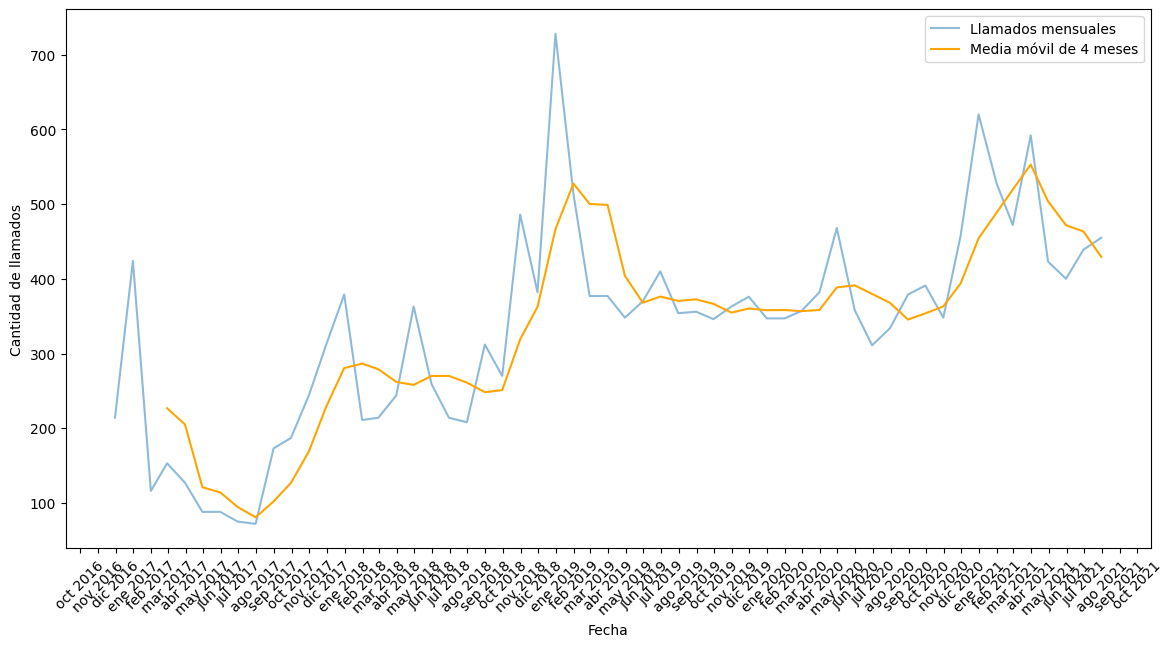
\includegraphics[scale=.5]{images/latex_trend_llamados.png}
    \caption{Cantidad de llamados en el tiempo con media móvil de 4 meses.}
    \label{trend}
    \end{center}
    \end{figure}

Además, construí las variables \textit{estación del año}, \textit{fin de semana}, y \textit{momento del día} para explorar la posibilidad de otros patrones en los llamados. Observé que una mayor proporción de llamados ocurren durante la semana (80\%) y por la tarde (38\%). No observé disparidad significativa en la distribución de llamados de acuerdo a las estaciones del año.


Según la distribución de la variable \textit{llamado\_provincia}, la mayoría de los llamados provienen de la Ciudad Autónoma (37\%) y la Provincia de Buenos Aires (36\%). Del 9\% no se cuentan con datos (respuestas \textit{NS/NC}); y el restante 18\% se reparte entre las restantes provincias del país, siendo de ese grupo Córdoba y Santa Fé las que más llamados tienen, con un 3\% cada una.\footnote{Ver figura \ref{provincia} en el \nameref{anex}.}

Según la distribución de la variable \textit{caso\_judicializado}, el 46.7\% de los llamados no está asociado a un caso ya judicializado, el 39.7\% sí, y en el restante 13.4\% no se cuenta con datos de este tipo.\footnote{Ver figura \ref{casojudicializado} en el \nameref{anex}.} 

En cuanto a la variable \textit{hecho\_lugar}, como ilustra el \textit{barplot} de la figura \Ref{hecholugar}, para aproximadamente el 30\% de los llamados no se cuenta con datos (respuestas \textit{NS/NC}); luego, el 25\% los hechos suceden en la vivienda de la víctima y el 13\% en la vivienda del agresor. La cuarta categoría más reportada, con el 12\%, es \textit{redes sociales}. El restante 20\% se divide entre categorías de espacios públicos (plazas, descampados, etc.), transporte, y ámbito educativo, entre otros sitios. La elevada proporción de casos que suceden en la vivienda de la víctima, es un dato que acompaña lo ya dicho en la \nameref{intro} sobre la mayoría de los hechos de violencia sexual ocurriendo más bien en el entorno de la víctima antes que involucrar personas y lugares desconocidos. 

\begin{figure}[H]
    \begin{center}
    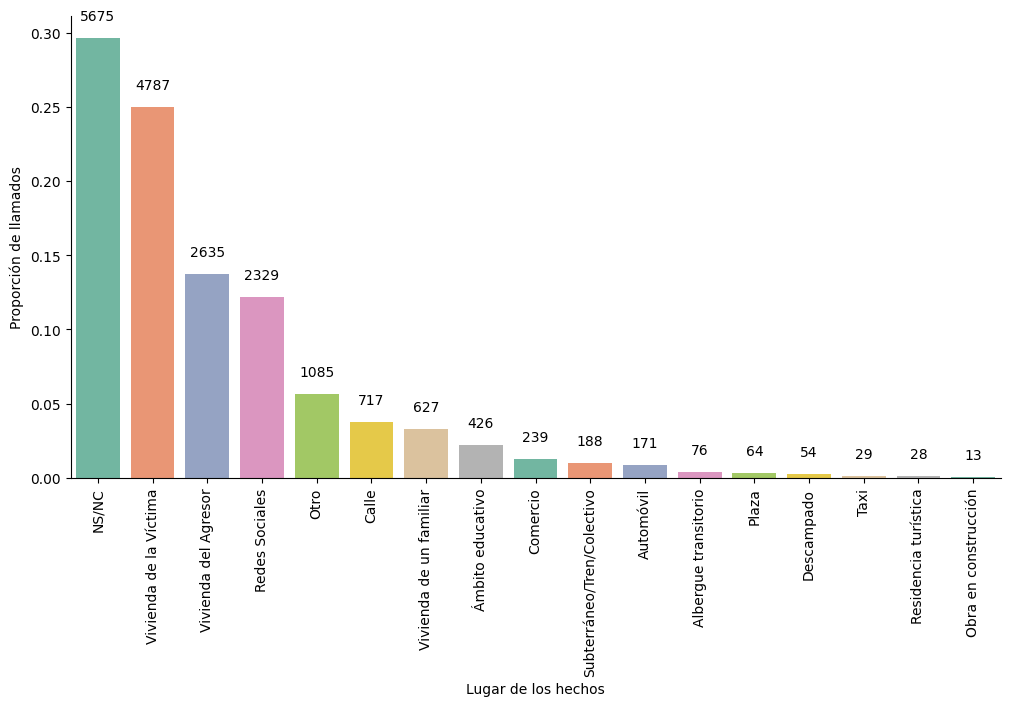
\includegraphics[scale=.5]{images/latex_lugar_hechos.png}
    \caption{Lugar de los hechos.}
    \label{hecholugar}
    \end{center}
    \end{figure}


Por otro lado, llama la atención la cuarta categoría más presente en \textit{hecho\_lugar}, los casos sucedidos en redes sociales. Para explorar este fenómeno, crucé en la figura \ref{redes}  esa categoría de \textit{hecho\_lugar} con los tipos de violencia sufrida y las edades de las víctimas agrupadas cualitativamente en Niñez (0 a 11 años), Adolescencia (12 a 18 años), Juventud (19 a 30 años), Adultez (31 a 65 años), y Vejez (mayores de 65). Observé que la mayor cantidad de casos corresponden al tipo de violencia \textit{grooming} en primer lugar, y en segundo lugar a la categoría \textit{ofv\_no\_sabe\_no\_contesta}. Además, aunque con conteos mucho más bajos, aparecen también otras formas de violencia esperables en el contexto de redes sociales como: \textit{ofv\_sentimiento\_amenaza}, \textit{vs\_explotacion\_sexual}, o \textit{ofv\_amenaza\_explicita}. En todos estos casos alrededor del 90\% de las víctimas son niñes o adolescentes. Si bien por la distribución de la variable \textit{victima\_edad} cabría esperar mayor cantidad de víctimas de estos grupos etarios, en el caso de los hechos sucedidos en redes sociales, este dato podría estar asociado con el mayor uso de redes sociales por parte de este sector de la población. 

\begin{figure}[H]
    \begin{center}
    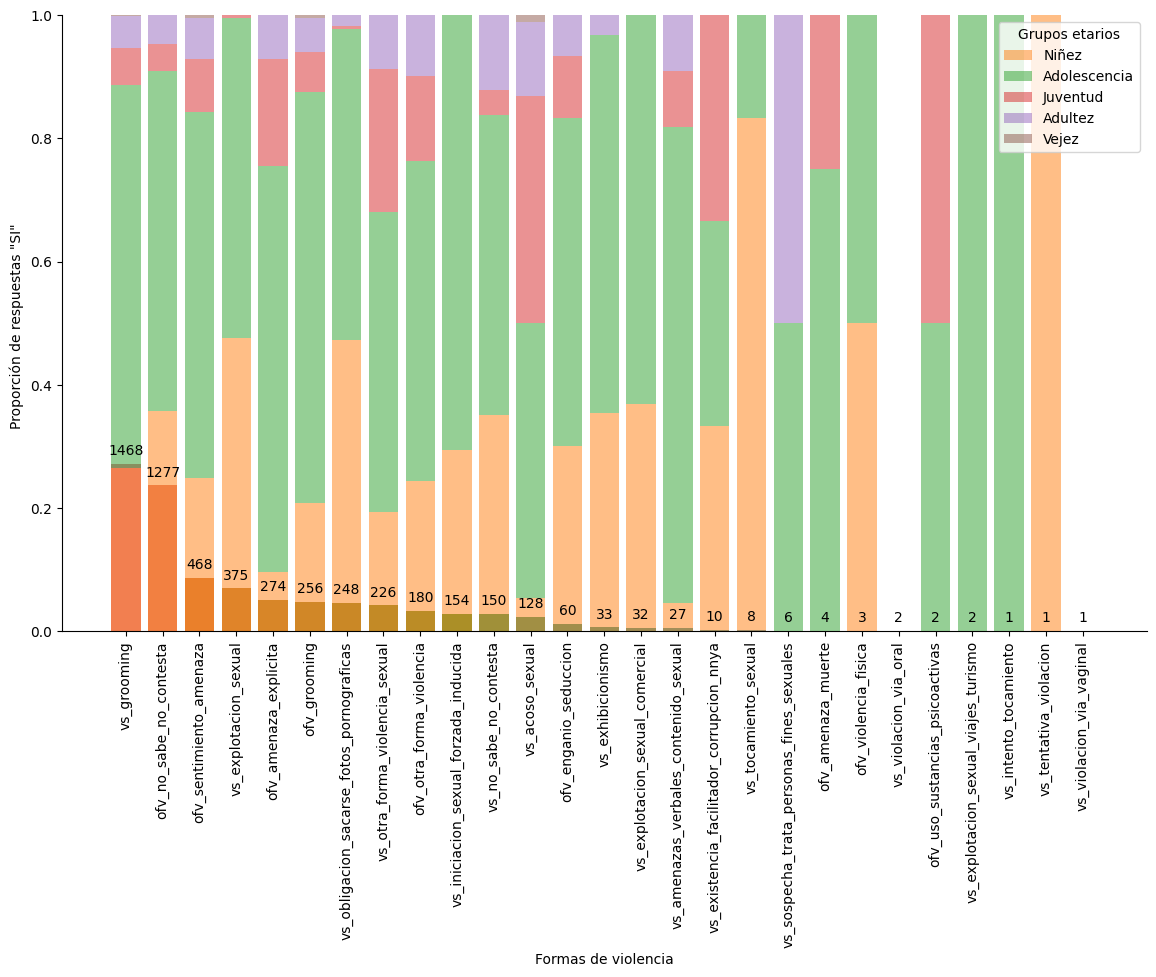
\includegraphics[scale=.5]{images/latex_redes_sociales_edad_formas_violencia.png}
    \caption{Proporción de “SI” en hechos de violencia ocurridos en redes sociales, agrupado por edad.}
    \label{redes}
    \end{center}
    \end{figure}


La nacionalidad de las víctimas, informada por \textit{victima\_nacionalidad}\todo[inline]{reduje víctima nacionalidad para SVM?}, se distribuye de la siguiente manera: el 80\% de las víctimas son argentinas; del 15\% no se cuenta con datos; y el restante 5\% se divide entre las nacionalidades boliviana, paraguaya, peruana, brasileña, uruguaya, chilena, y la categoría “otra”.\footnote{Ver figura \ref{nacionalidad} en el \nameref{anex}
}


Según la distribución de \textit{victima\_discapidad}, para el 53.7\% de las víctimas no se cuenta con datos, el 43.2\% no posee discapacidad, y el 2.9\% sí\footnote{Ver figura \ref{discapacidad} en el \nameref{anex}}. 


En el \textit{barplot} de la figura \Ref{genero}, se ve reforzado el dato mencionado en la introducción sobre la distribución de género de las víctimas: el 77.6\% de las víctimas son mujeres, el 18.4\% hombres, del 3.7\% no se tienen datos, y el 0.14\% son personas tránsgenero. 

\begin{figure}[H]
    \begin{center}
    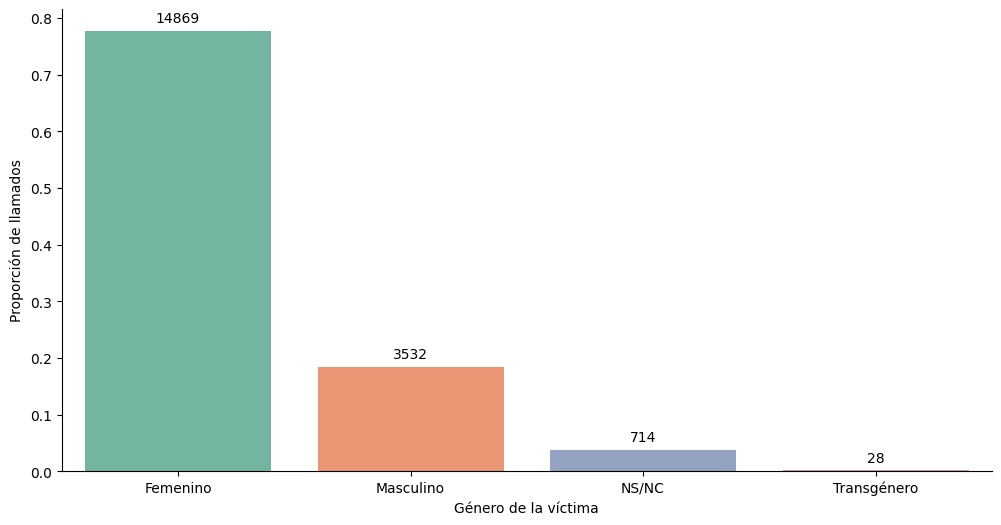
\includegraphics[scale=.5]{images/latex_genero_victima.png}
    \caption{Género de las víctimas.}
    \label{genero}
    \end{center}
    \end{figure}

Los vínculos entre víctimas y agresores nuevamente reflejan la persistencia de los hechos de violencia sexual perpetuados por personas del entorno de las víctimas. En el gráfico de barras de la figura \Ref{vinculoagresor} para la variable \textit{victima\_vinculo\_agresor} se observa la distribución en las diferentes categorías vinculares. Pero además la tendencia se evidencia aún más al reagrupar las categorías de la variable en \textit{Conocido familiar}, \textit{Conocido no familiar} (categoría ya presente en la variable original) \textit{Desconocido}, y \textit{NS/NC}. Mientras que 15.4\% de los agresores son declarados como desconocidos; entre familiares (47.4\%) y no familiares (19.7\%), los agresores conocidos por la víctima suman un 67.1\%. El número podría incluso ser más elevado si consideramos que podría haber agresores conocidos también como parte del 17.2\% de los \textit{NS/NC}.



\begin{figure}[H]
    \begin{center}
    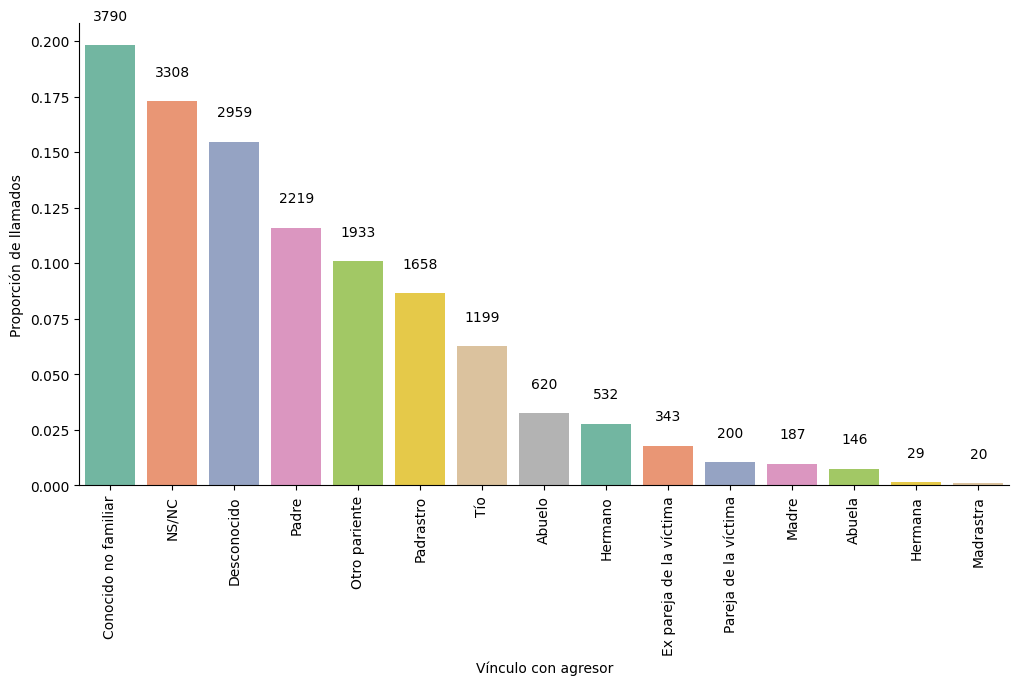
\includegraphics[scale=.5]{images/latex_vinculo_agr_victima.png}
    \caption{Vínculos víctima-agresor.}
    \label{vinculoagresor}
    \end{center}
    \end{figure}

    \begin{figure}[H]
        \begin{center}
        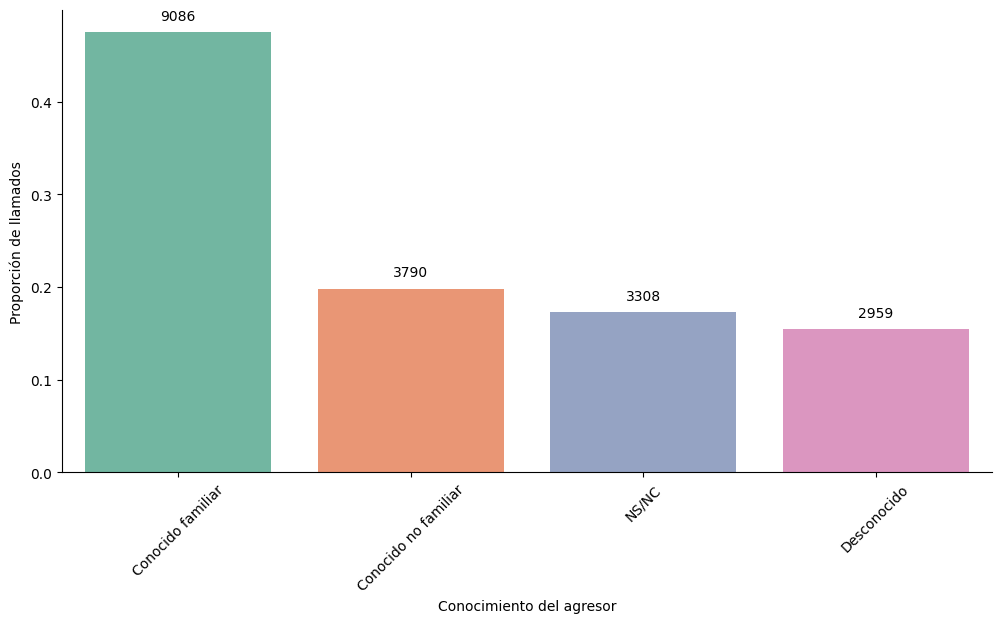
\includegraphics[scale=.5]{images/latex_agresor_conocido_no.png}
        \caption{Agresor conocido o no por la víctima.}
        \label{conocidodesconocido}
        \end{center}
        \end{figure}




 En la variable \textit{vinculo\_llamante\_victima}, el 24.9\% de los llamados provienen de comisarías, el 17.2\% de un familiar de la víctima (otro familiar que no pertenezca a las categorías: \textit{Madre}, \textit{Padre}, \textit{Abuela/o}, o \textit{Hermana/o}), el 16\% de los llamantes son madres de las víctimas, y el 14.2\% lo constituyen las propias víctimas. El resto de las categorías son otros conocidos de las víctimas, padres, vecinos, abuelos, hermanos, otras instituciones, o \textit{NS/NC} todas con menos del 10\%. Por último, los llamados provenientes de escuelas, defensorías y los mismos agresores suman menos del 1\%.  \footnote{Ver figura \ref{vinculollamante} en el \nameref{anex}}



En cuanto a la variable de interés \textit{victima\_convive\_agresor}, encontré en el análisis univariado que un 64.4\% no convive, frente al 14.3\% que sí lo hace. Para el restante 21.19\% las respuestas son \textit{NS/NC}, y es la categoría que más adelante modelo como dato faltante para intentar predecir como \textit{SI} o \textit{NO}(ver firgura \Ref{convivencia}).  


\begin{figure}[H]
    \begin{center}
    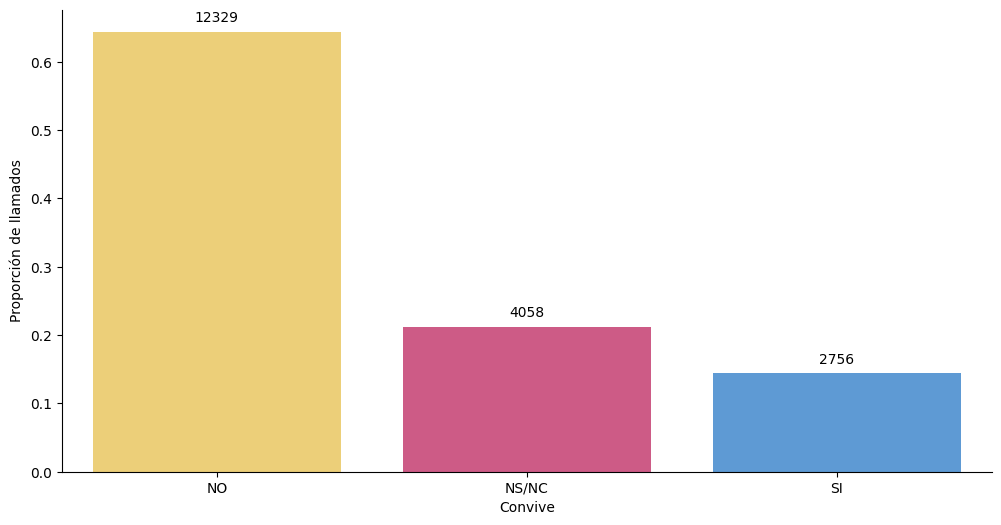
\includegraphics[scale=.5]{images/latex_convive.png}
    \caption{Convivencia víctima-agresor.}
    \label{convivencia}
    \end{center}
    \end{figure}



En la figura \ref{boxplotsconvivenciaedad} y el cuadro \ref{cuartilesconviveedad} se pueden ver \textit{boxplots} comparativos y un detalle del análisis de cuartiles de \textit{victima\_edad} según cada categoría de \textit{victima\_convive\_agresor}. Las víctimas que conviven con el agresor son ligeramente más jóvenes que las que no lo hacen, y las víctimas de las que no se cuentan con datos sobre la convivencia parecen estar más cerca en edad de las que conviven. Sin embargo, las diferencias en edad entre las víctimas que conviven y las que no que se reflejan tanto en los \textit{boxplots} como en el cuadro no parecen significativas\footnote{Realizo en la sección \nameref{met} un análsis más detallado con respecto a la correlación estadística entre la edad de la víctima y la variable de convivencia, entre otras.}. 

\begin{figure}[H]
    \begin{center}
    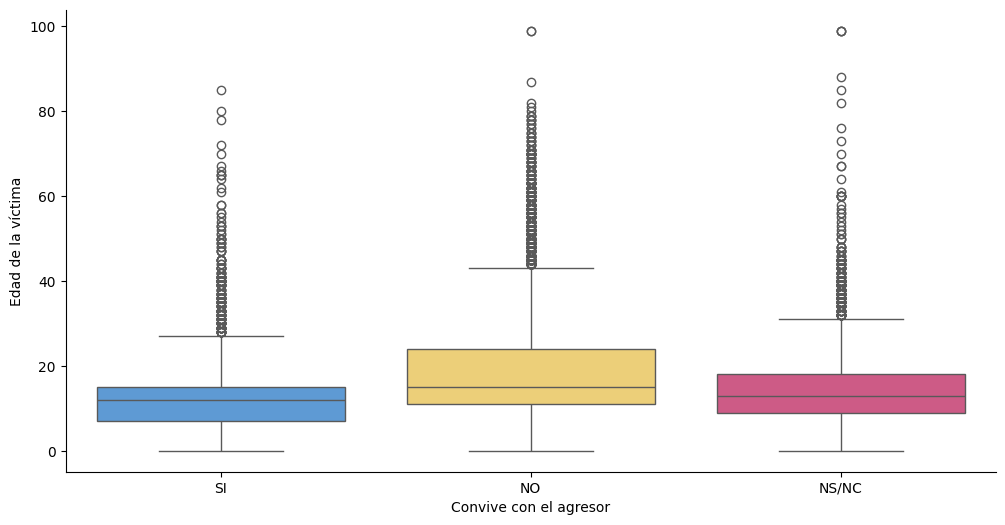
\includegraphics[scale=.5]{images/latex_boxplot_convive_edad.png}
    \caption{Distribución de la edad de la víctima según su convivencia o no con el agresor.}
    \label{boxplotsconvivenciaedad}
    \end{center}
    \end{figure}



\begin{table}[H]
    \begin{center}
    \caption{Cuartiles de edad según categoría de \textit{victima\_convive\_agresor}.}
    \label{cuartilesconviveedad}
    \begin{tabular}{cccc}
    \hline
    \multicolumn{1}{r}{\textbf{}} & \textbf{Convive} & \textbf{No Convive} & \textbf{ NS/NC} \\ \hline
    Q1                            & 7                    & 11                   & 9                       \\
    Q3                            & 15                   & 24                   & 18                      \\
    IQR                           & 11                   & 11                   & 11                     \\ \hline
    \end{tabular}
    \end{center}
    \end{table}


Exploré visualmente también la relación entre \textit{victima\_convive\_agresor}, y \textit{llamante\_vinculo}, \textit{hecho\_lugar}, \textit{momento\_dia}, y \textit{caso\_judicializado} porque podían estar relacionadas con la situación convivencial de la víctima y el agresor. Observé que la tendencia que se observa en la figura \Ref{convivencia}: mayoría de respuestas \textit{NO} y minoría de \textit{SI}, con \textit{NS/NC} posicionado ordinalmente en el medio de ambas, se mantiene en general constante en relación con estas variables. La única excepción, cono puede verse en la figura \ref{llamvincconvive}, es en la categoría \textit{vecina/o} de \textit{llamante\_vinculo} donde la tendencia de respuestas positivas y negativas se invierte: 48.4\% \textit{SI}, y 21.7\% \textit{NO}. Sobre esta variable observé también que los valores de \textit{NS/NC} para \textit{victima\_convive\_agresor} son notablemente más altos cuando el llamado proviene de \textit{Otra institución} que no sea una escuela, comisaría, u hospital. \footnote{En el \nameref{anex}  se pueden consultar las figuras \ref{hecholugconvive}, y \ref{momdiaconvive}, y \ref{casojudconvive} correspondientes a la relación entre \textit{victima\_convive\_agresor} y \textit{hecho\_lugar}, \textit{momento\_dia}, y \textit{caso\_judicializado}.}

\begin{figure}[H]
\begin{center}
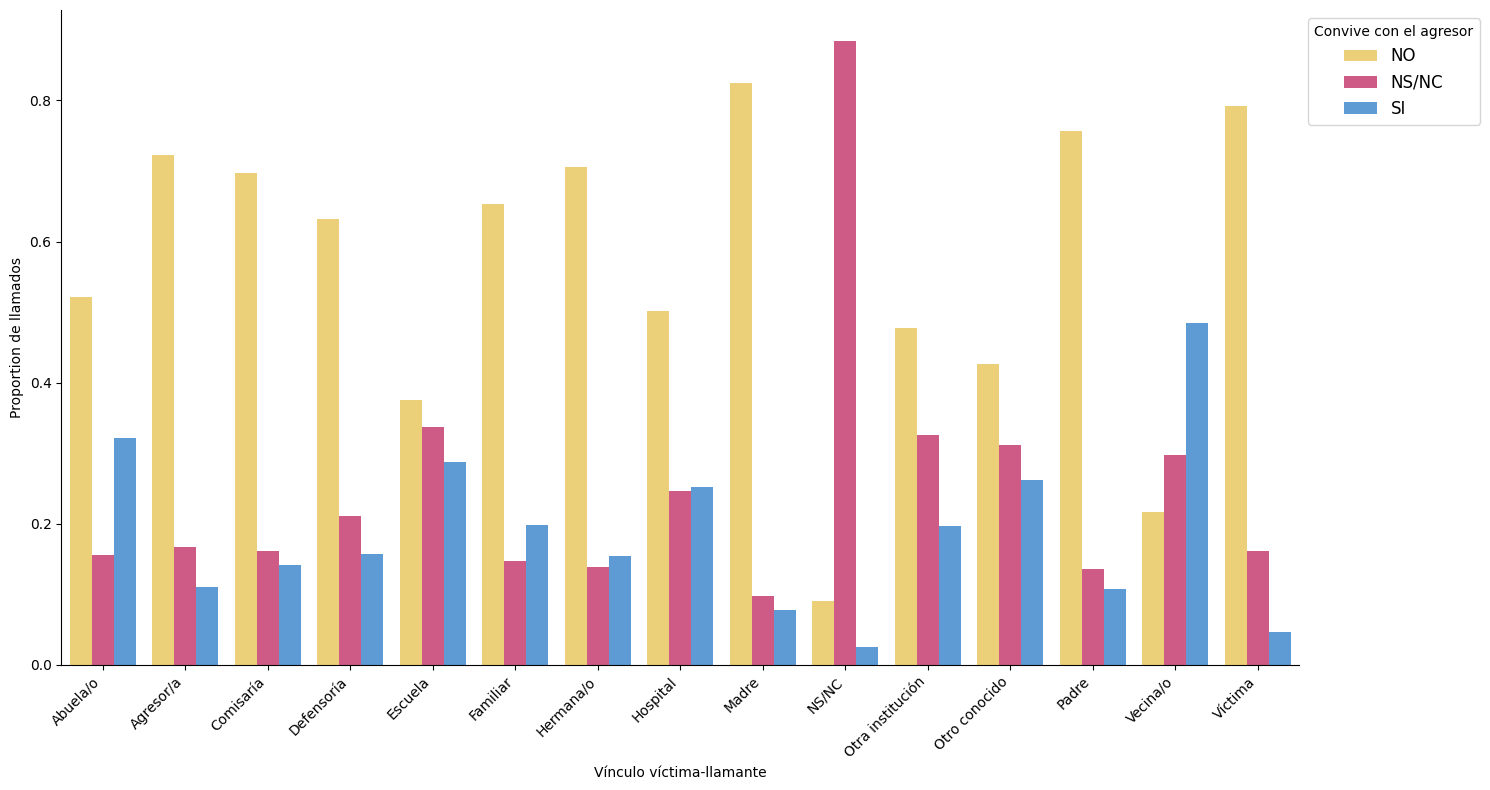
\includegraphics[scale=.5]{images/latex_llamante_vin_convive.png}
\caption{Convivencia con el agresor según vínculos víctima-llamante.}
\label{llamvincconvive}
\end{center}
\end{figure} 


Las variables que describen la violencia sexual sufrida y otras formas de violencia reportadas solo toman en este conjunto de datos los valores \textit{SI} y \textit{NO}. Además, todas presentan en general más cantidad de respuestas negativas que positivas. A continuación, en las figuras \ref{vssino} y \ref{ofvsino} se puede apreciar la distribución de respuestas para violencia sexual y otras formas de violencia respectivamente. Es interesante notar que las categorías de “no sabe/no contesta” son la segunda con más respuestas en formas de violencia sexual y la primera con más respuestas en otras formas de violencia. Es decir, en gran cantidad de llamados se reporta una forma de violencia (sexual o no) sufrida, pero no se puede reportar qué forma. 

\begin{figure}[H]
\begin{center}
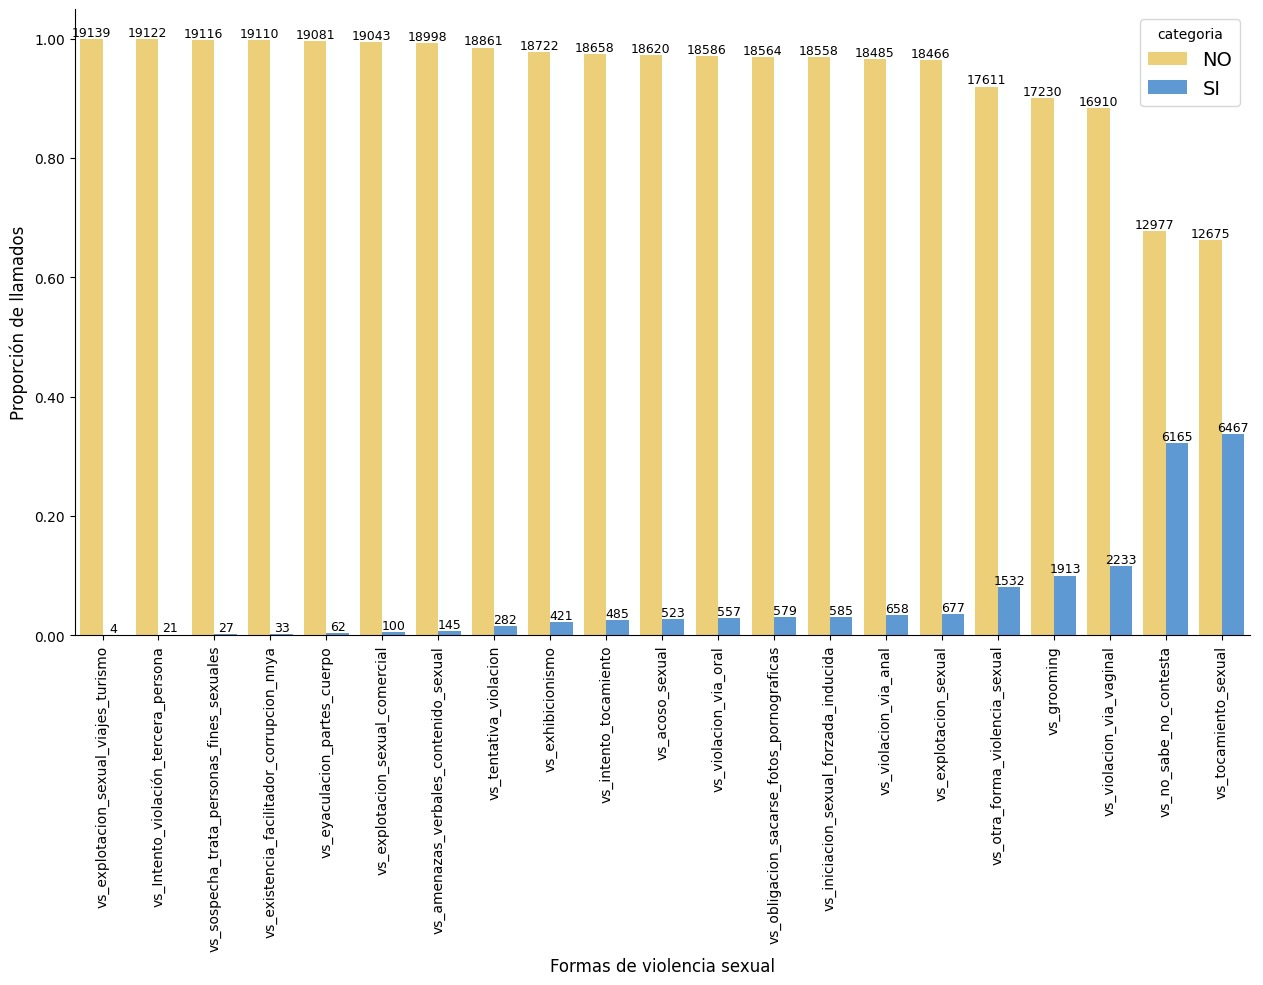
\includegraphics[scale=.5]{images/latex_vs_sino.jpeg}
\caption{Tipos de violencia sexual reportada en los llamados.}
\label{vssino}
\end{center}
\end{figure} 

\begin{figure}[H]
\begin{center}
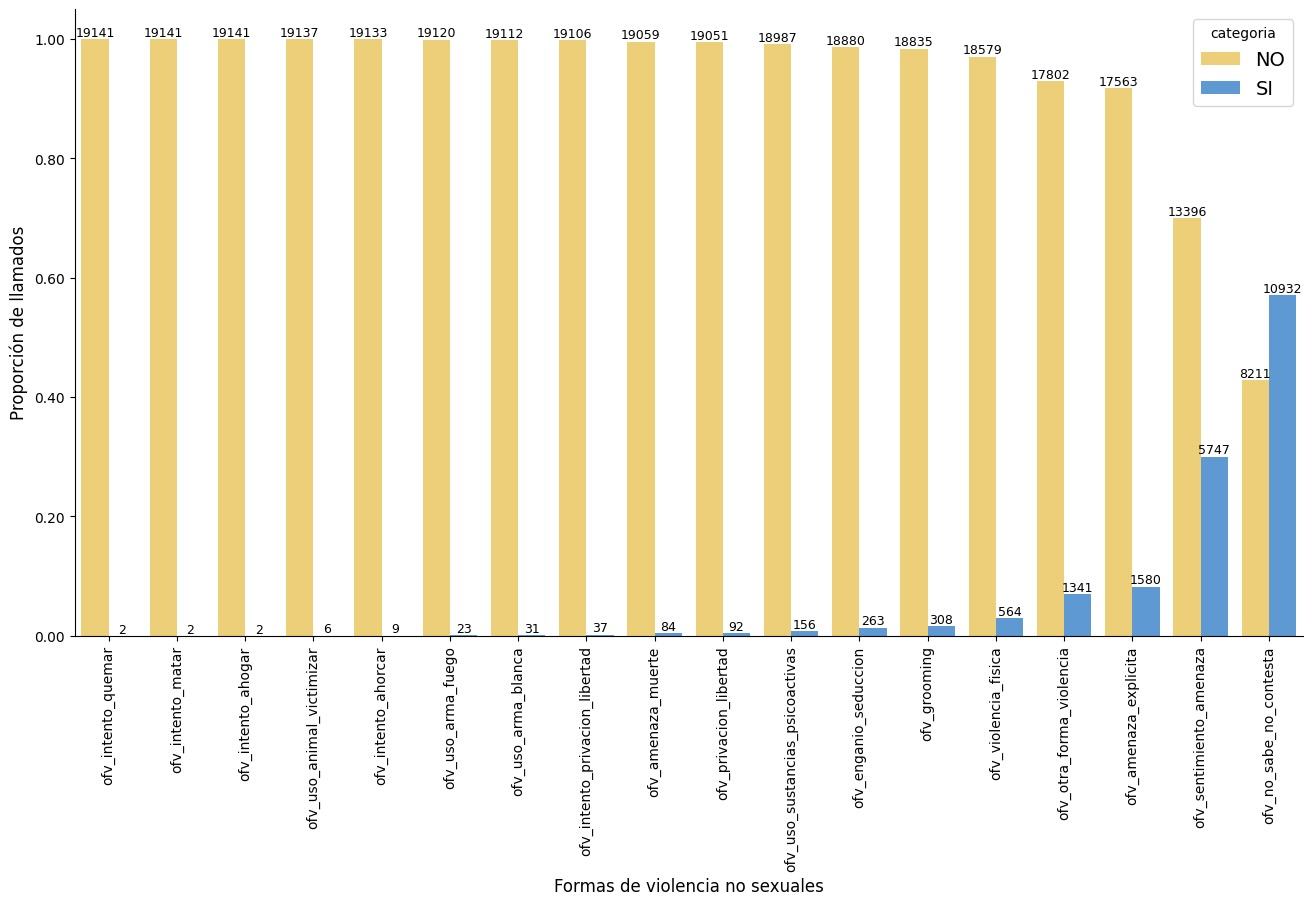
\includegraphics[scale=.5]{images/latex_ofv_sino.jpeg}
\caption{Tipos de violencia no sexual reportada en los llamados.}
\label{ofvsino}
\end{center}
\end{figure} 


\subsection*{Datos faltantes}\label{faltantes}

Los datos faltantes se presentan en este conjunto de datos como efectivamente faltantes, es decir, sin valores cargados, solo en las variables de edad. Donde en edad de la víctima representan el 9.82\%, y en la edad de quien llama el 44.82\%. 
En la variable de interés \textit{victima\_convive\_agresor}, no hay celdas con valores ausentes. Como ya expresé más arriba, sin embargo, el objetivo de este trabajo es clasificar las respuestas \textit{NS/NC} como \textit{SI} o \textit{NO}. Por lo tanto, considero ese tipo de respuestas, que representan el 21.19\%, como datos faltantes que deberían ser completados con respuestas positivas o negativas.

el ordenamiento original es NO > NS/NC > SI
s/d edad victima: NS/NC > NO > SI NS/NC se incrementa en un 30% más o menos. Decrece mucho NO y un poco SI. Es decir, realmente no saben.


posible relación de datos faltantes de edad con quien llama tanto en edad de la victima como en edad de quien llama
relación entre los faltante de edad y NSNC en convive

relaci;on entre NSNC de convive y quien llama (instituciones) esto está en la notebook de por qué faltan mis datos y en las notas que tomé

por qué faltan? la respuestas más senciulla es que simplemente algunos datos no se conocen, el llamante puede no saber realmente la edad de la víctima o si convive o no, etc. Otra causa puede ser la necesidad de oculktar ciertos datos por estigma o por protección de la víctima, de su entorno o incluso del agresor. la realidad como sucede con los datos faltabtes de este tipo, es que es imposible saber el motivo real por el que falten y puede que sea una combinación de todas esas razones.


\section*{Metodología}\label{met}

El objetivo es imputar los NS/NC de convive como si o no. 

Intento ver si usando un método de ordenamiento para visualizar el dataset en dimensiones reducidas me da una
idea de agrupamientos con repsecto a las tres categorías de convive. Elijo NMDS porque me permite trabajar con
variables de distinto tipo sin transformaciones.
 Luego, para intentar predecir los NSNC como si o no usé SVM. 

A modo de un segundo preprocesamiento para poder llevar a cabo estas tareas, decidí reducir las dimensiones del dataset a mano primero agrupando variables y reduciendo la cantidad de categorías en algunas otras variables. lA REDUCCI´OND E CARDINALIDAD DE algunas variables es especialemnte útil para la aplicación de SVM ya que esta conlleva encodear las features y para uno de los encoders elegidos, one-hot, la alta cardinalidad de features puede resultar problemática.


Habiendp hecho los gráficos de más arriba para explorar posibles interacciones entre dos o tres variables, me pareció valioso explorar más dimensiones y plasmarlo en dos dimensiones. Para eso apliqué NMDS

Reducción manual de dimensiones
Algunas resultan muy poco informativas como vs explotacion sexual viajes turismo (0,02) y ofv intento matar (0,01) resultan muy poco informativas (ocurrencia de 0,02 y 0,01). 

Despues medí correlación para ver si podía sacar más variables pero al final no saqué ninguna. Explicar cómo queda el dataset final

Después apliqué encoders para hacer SVM e hice SVM con la librería tal y con una búsqueda de hiperparámetros. Además experimenté con diferentes versiones del dataset cambiando la variable edad numérica por su contraparte categórica. Esto me peritió medir el posible impacto de los datos faltantes de edad. Cuando la edad era numérica, debía dejar afuera los datos faltantes ya que SVM no puede utilizarlos. Para poder utilizar todos los datos completos de edad, pasé la edad a categorica  utilizando las categorías tal tal y tal y dejado como NSNC los datos faltantes. Teniendo en cuenta estas variaciones en el tratamiento de la variable edad, los experimentos que realicé con SVM fueron: 
tal tal tal

cada uno probando los siguientes hiperparámentros

VER DE ARMAR UNA TABLA QUE RESUMA ESTAS VARIANTES 


\section*{Resultados}\label{resultados}
NMDS vemos que no hay en ninguna de las veriones del dtaset que usé una separación clara entre las categorías de interés.

VER DE RE ARMAR NMDS y que separe solo SI de NO y luego un tercero que haga SI NO NSNC

Todos dieron bien y luego el mejor modelo lo apliqué a 

\section*{Discusión y conclusiones}\label{conc}
cruzamiento de datos ovd líneas de asistencia, observatorio de género.
acceso y análisis de datos extensivo a provincias, no solo benos aitres


VER DE EN SVM RESULTANTE FINAL A LOS QUE LES PUSO S´I CU´AL ES LA EDAD DE V´ICTIMA Y A LOS QUE LES PUSO NO, CU´AL ES

en \textit{La guerra contra las mujeres}, \citeyearpar{segato2016guerra}, Rita Segato habla de la violencia sexual como algo siempre dirigido hacia cuerpos femeninos y \textit{feminizados} (resaltado propio). Con esto último quiere decir cuerpos percibidos o construidos por los abusadores como femeninos con respecto a posiciones de poder: menores, débiles, racializados, pertenecientes a disidencias sexuales. Esto se condice con datos sobre la mayor incidencia de la violencia sexual contra identidades masculinas durante la niñez y la adolescencia, es decir, en períodos en que los cuerpos y los sujetos son más vulnerables, y por lo tanto, también percibidos como feminizados \citep*{contreras2016violencia,ufem_relevamiento,ferris2002world}.

Si las denuncias de violencia sexual contra disidencias de género representan una minoría en los datos, ¿quiere decir esto que esas personas sufren menos violencia sexual?, ¿O quiere decir que, como minoría social, están subrepresentados en general y que tienen menos acceso a la justicia?



Análisis de series temporales, porsibilidad de hacer forcasting
\newpage


\bibliography{bibtex_reporte.bib}

\newpage
\section*{Anexo}\label{anex}




\begin{figure}[H]
\begin{center}
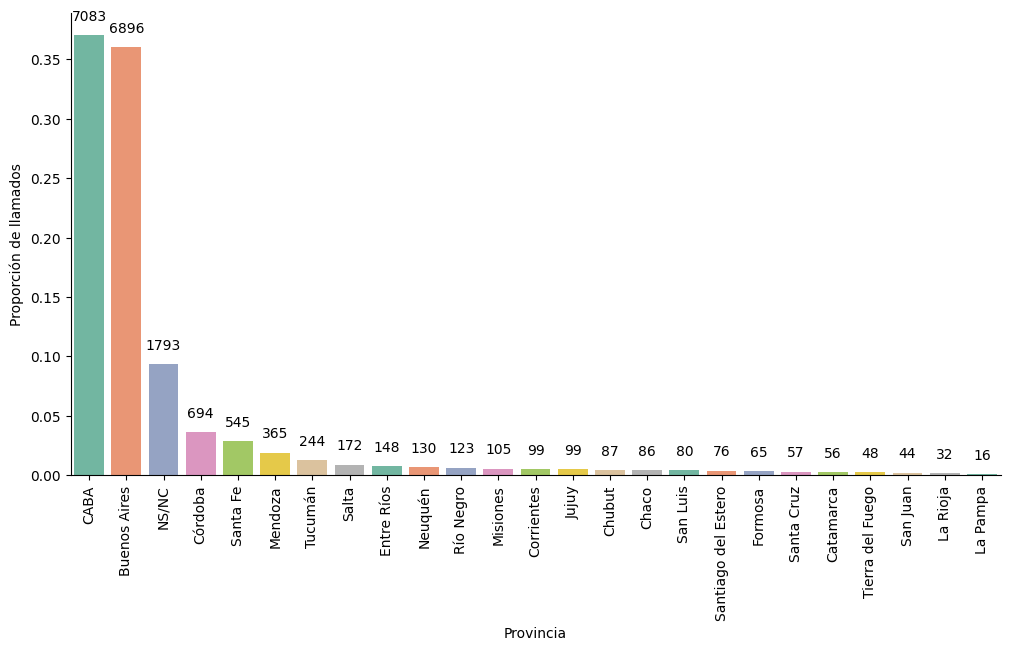
\includegraphics[scale=.5]{images/latex_llamados_por_provincia.png}
\caption{Llamados por provincia.}
\label{provincia}
\end{center}
\end{figure}

\begin{figure}[H]
\begin{center}
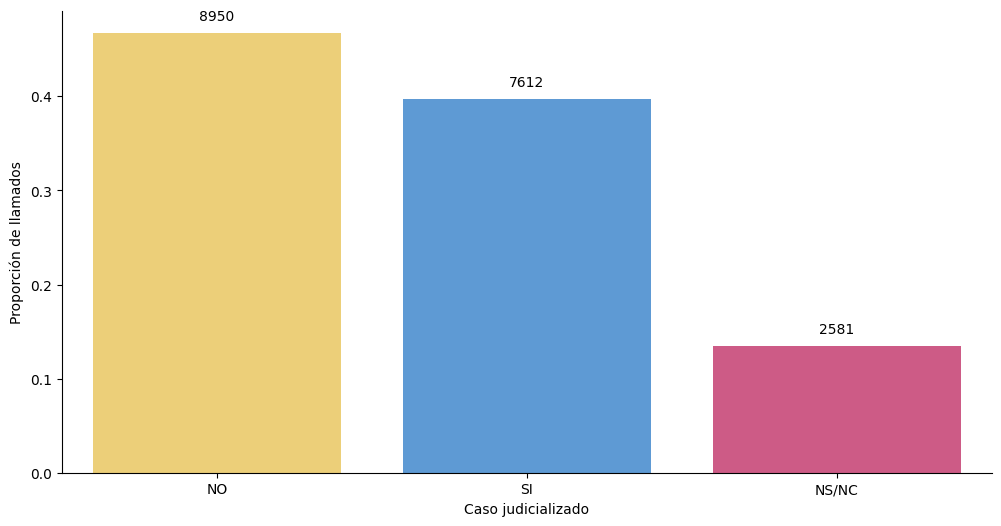
\includegraphics[scale=.5]{images/latex_caso_judicializado.png}
\caption{Caso judicializado.}
\label{casojudicializado}
\end{center}
\end{figure}


\begin{figure}[H]
\begin{center}
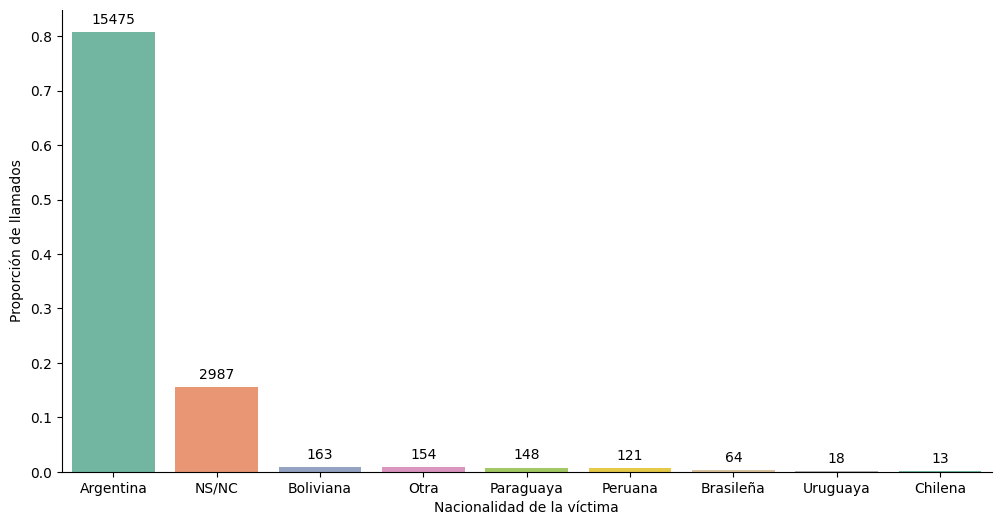
\includegraphics[scale=.5]{images/latex_nacionalidad_victima.png}
\caption{Nacionalidad de las víctimas.}
\label{nacionalidad}
\end{center}
\end{figure}



\begin{figure}[H]
\begin{center}
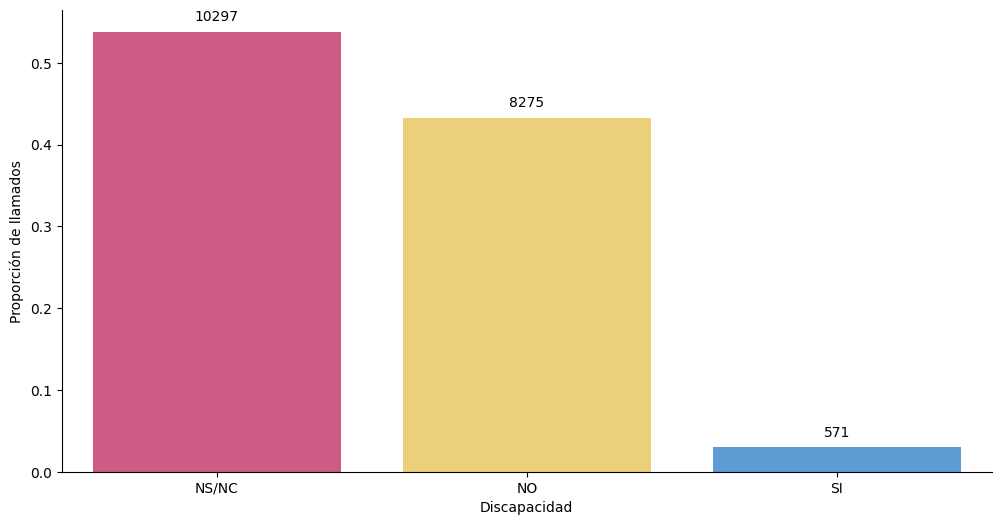
\includegraphics[scale=.5]{images/latex_victima_discapacidad.png}
\caption{Presencia de discapacidad en las víctimas.}
\label{discapacidad}
\end{center}
\end{figure}



\begin{figure}[H]
\begin{center}
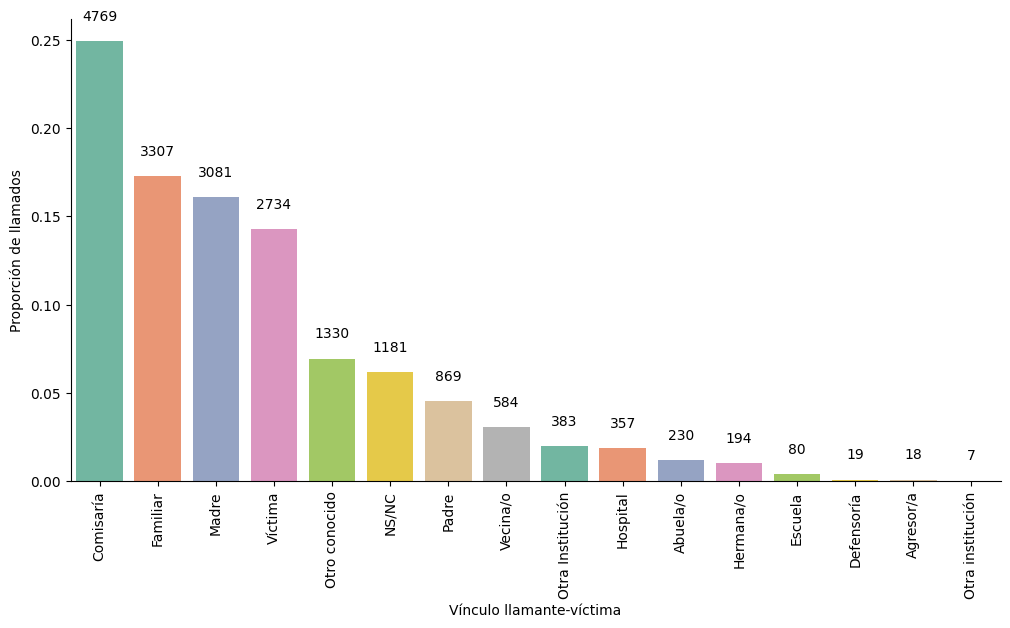
\includegraphics[scale=.5]{images/latex_vinculo_llamante.png}
\caption{Vínculos víctima-llamante.}
\label{vinculollamante}
\end{center}
\end{figure}

       

\begin{figure}[H]
\begin{center}
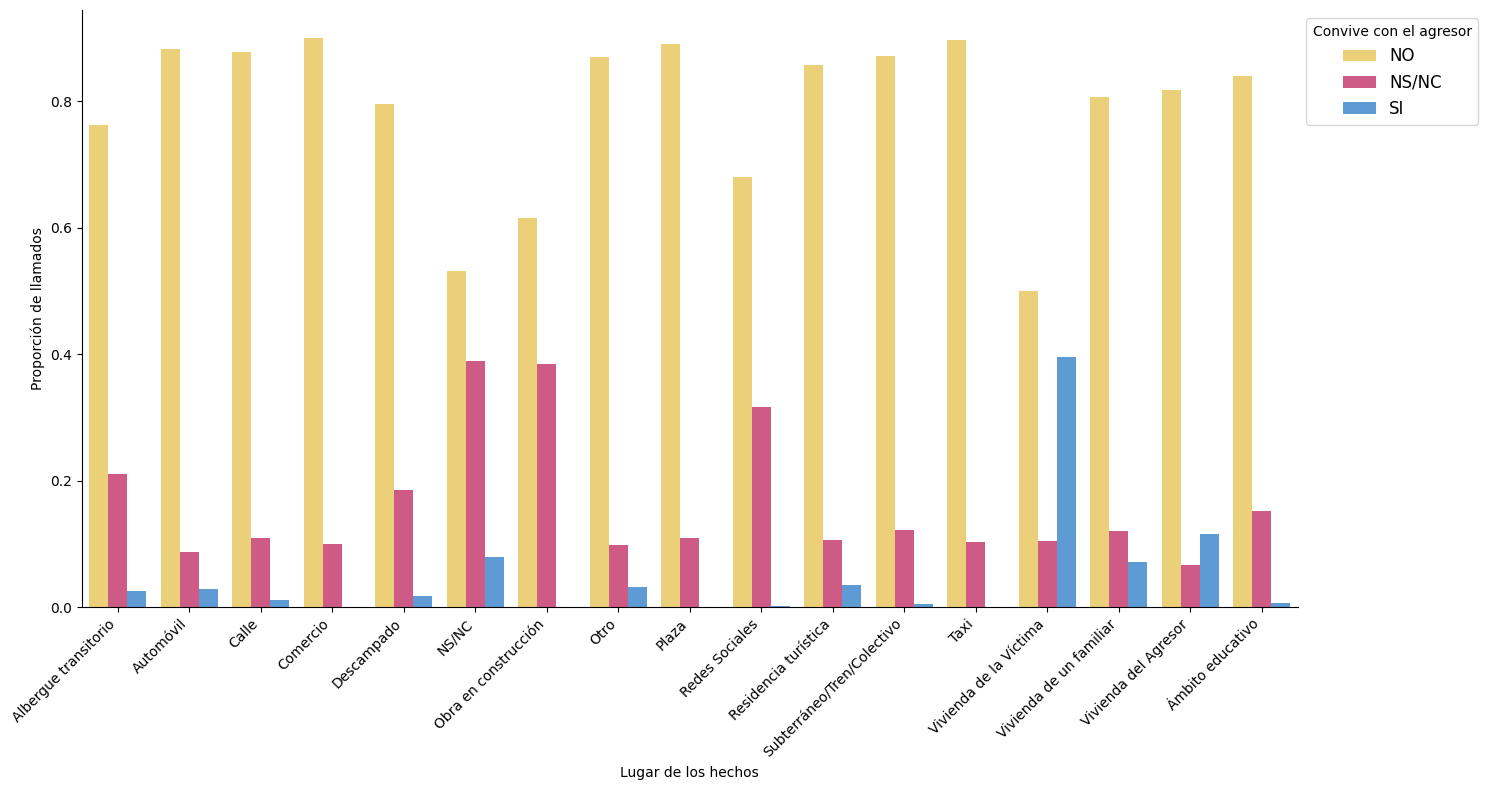
\includegraphics[scale=.5]{images/latex_hecho_lugar_convive.png}
\caption{Convivencia con el agresor según lugar de los hechos.}
\label{hecholugconvive}
\end{center}
\end{figure}

\begin{figure}[H]
\begin{center}
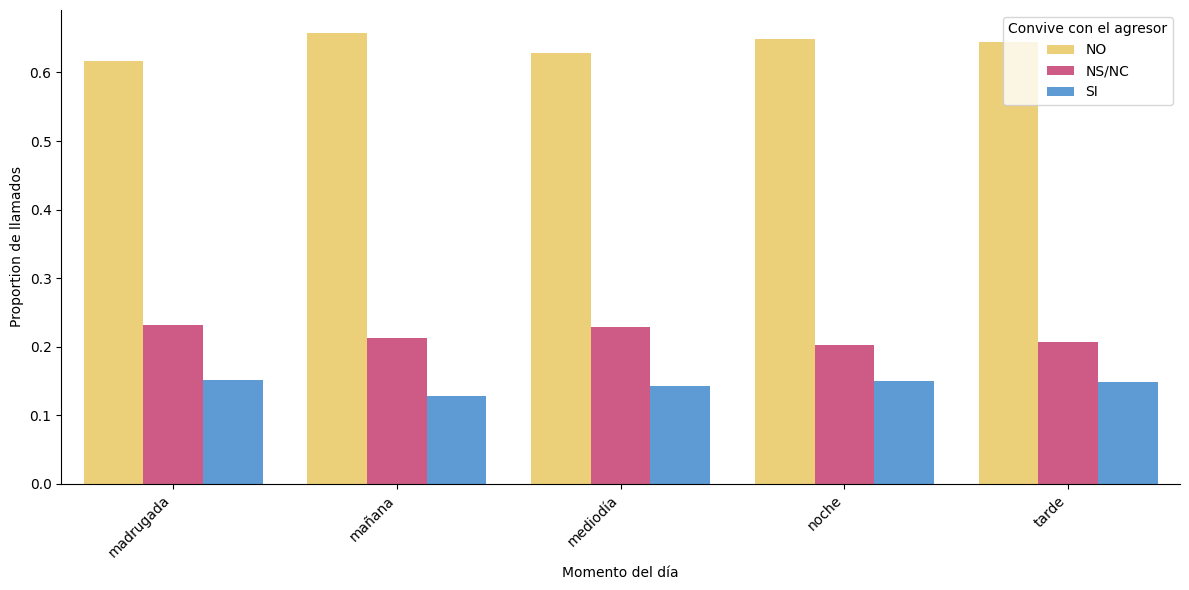
\includegraphics[scale=.5]{images/latex_momento_dia_convive.png}
\caption{Convivencia con el agresor según momento del día del llamado.}
\label{momdiaconvive}
\end{center}
\end{figure}

\begin{figure}[H]
\begin{center}
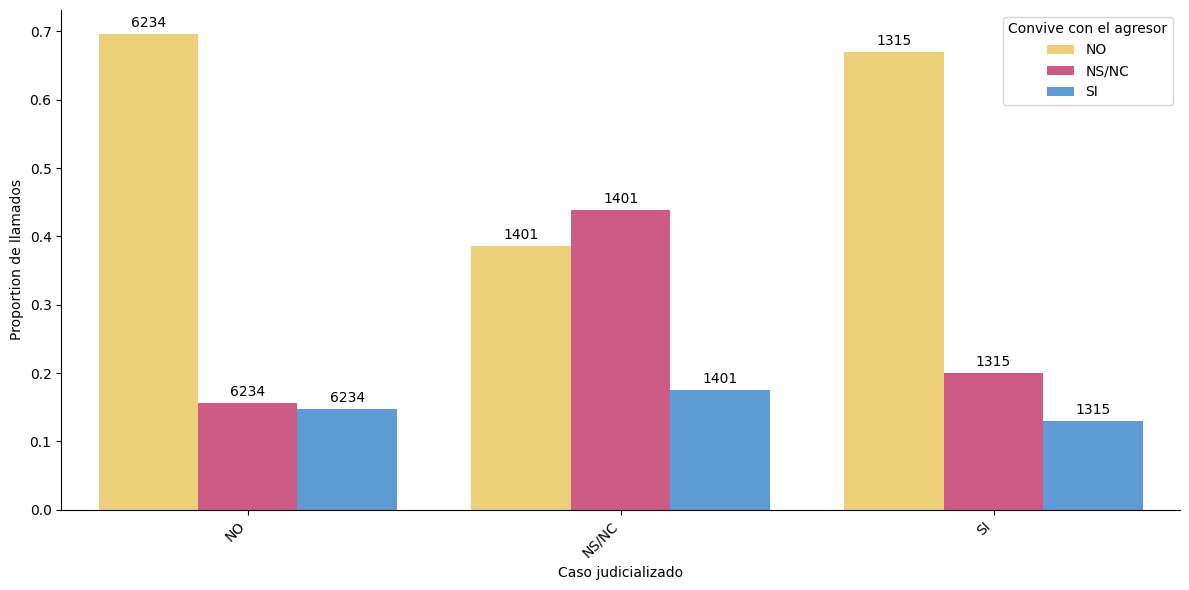
\includegraphics[scale=.5]{images/latex_caso_jud_convive.png}
\caption{Convivencia con el agresor según estado judicial del caso.}
\label{casojudconvive}
\end{center}
\end{figure}

\end{document}